\subsection{Упражнение 1}

Убедимся в том, что analyze1 требует времени пропорционально n^3, а analyze2 пропорционально n^2. Для этого будем запускать их с несколькими разными массивами и засекать время работы при помощи команды %timeit

\begin{lstlisting}[language=Python]
def analyze1(ys, fs, ts):
    args = np.outer(ts, fs)
    M = np.cos(PI2 * args)
    amps = np.linalg.solve(M, ys)
    return amps
    
def analyze2(ys, fs, ts):
    args = np.outer(ts, fs)
    M = np.cos(PI2 * args)
    amps = M.dot(ys) / 2
    return amps
\end{lstlisting}

Возьмем сигнал шума и массив, состоящий из степеней двойки

\begin{lstlisting}[language=Python]
from thinkdsp import UncorrelatedGaussianNoise

signal = UncorrelatedGaussianNoise()
noise = signal.make_wave(duration = 1.0, framerate = 8192)
noise.ys.shape

(8192,)
\end{lstlisting}

\begin{lstlisting}[language=Python]
ns = 2 ** np.arange(6, 14)
ns

array([  64,  128,  256,  512, 1024, 2048, 4096, 8192])
\end{lstlisting}

Напишем функцию plot_bests, которая будет брать массив результата из эксперимента и строить график

\begin{lstlisting}[language=Python]
from scipy.stats import linregress

def plot_bests(bests):
    plt.plot(ns, bests)
    loglog = dict(xscale='log', yscale='log')
    decorate(xlabel='Wave length (N)', ylabel='Time (s)', **loglog)
    x = np.log(ns)
    y = np.log(bests)
    t = linregress(x, y)
    slope = t[0]

    return slope
\end{lstlisting}

Вычисдим результат для analyze1

\begin{lstlisting}[language=Python]
results = []
for N in ns:
    print(N)
    ts = (0.5 + np.arange(N)) / N
    freqs = (0.5 + np.arange(N)) / 2
    ys = noise.ys[:N]
    result = %timeit -r1 -o analyze1(ys, freqs, ts)
    results.append(result)

bests = [result.best for result in results]
plot_bests(bests)

64
The slowest run took 4.21 times longer than the fastest. This could mean that an intermediate result is being cached.
1000 loops, best of 1: 243 µs per loop
128
1000 loops, best of 1: 818 µs per loop
256
100 loops, best of 1: 3.57 ms per loop
512
100 loops, best of 1: 18.1 ms per loop
1024
10 loops, best of 1: 73.7 ms per loop
2048
1 loop, best of 1: 549 ms per loop
4096
1 loop, best of 1: 3.68 s per loop
8192
1 loop, best of 1: 24.4 s per loop
2.3906127505491934
\end{lstlisting}

\begin{figure}[H]
	\begin{center}
		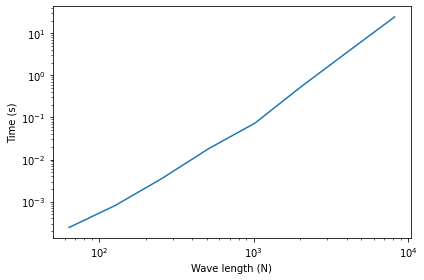
\includegraphics[scale=1]{fig/lab06/lab06_01.png}
		\caption{Время работы метода ДКП analyze1}
	\end{center}
\end{figure}

Исходя из графика видно, что расчетный наклон близок к 2, а не 3, как ожидалось. Также на графике видно, что в конце линия немного изогнута, что говорит о том, что размер массива не достигнут, где analyze1 будет пропорционально n^3. Получается, что при больших размерах массива, рост analyze1 будет пропорционален n^3, а так он ближе к n^2

Теперь протестируем analyze2

\begin{lstlisting}[language=Python]
signal = UncorrelatedGaussianNoise()
noise = signal.make_wave(duration = 1.0, framerate = 8192)
noise.ys.shape

(8192,)

ns = 2 ** np.arange(6, 14)
ns

results = []
for N in ns:
    print(N)
    ts = (0.5 + np.arange(N)) / N
    freqs = (0.5 + np.arange(N)) / 2
    ys = noise.ys[:N]
    result = %timeit -r1 -o analyze2(ys, freqs, ts)
    results.append(result)

bests2 = [result.best for result in results]
plot_bests(bests2)
array([  64,  128,  256,  512, 1024, 2048, 4096, 8192])

64
10000 loops, best of 1: 99.1 µs per loop
128
1000 loops, best of 1: 558 µs per loop
256
100 loops, best of 1: 8.5 ms per loop
512
100 loops, best of 1: 14.8 ms per loop
1024
10 loops, best of 1: 41.4 ms per loop
2048
10 loops, best of 1: 134 ms per loop
4096
1 loop, best of 1: 401 ms per loop
8192
1 loop, best of 1: 1.49 s per loop
1.8809074973380902
\end{lstlisting}

\begin{figure}[H]
	\begin{center}
		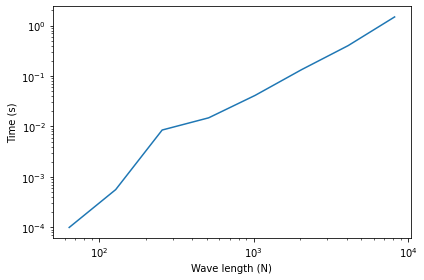
\includegraphics[scale=1]{fig/lab06/lab06_02.png}
		\caption{Время работы метода ДКП analyze2}
	\end{center}
\end{figure}

Исходя из графика видно, что analyze2 растет пропорционально n^2, как и ожидалось

Теперь проведем такой же эксперимент с использованием scipy.fftpack.dct

\begin{lstlisting}[language=Python]
from scipy.fftpack import dct

results = []
for N in ns:
    print(N)
    ts = (0.5 + np.arange(N)) / N
    freqs = (0.5 + np.arange(N)) / 2
    ys = noise.ys[:N]
    result = %timeit -r1 -o dct(ys, type = 3)
    results.append(result)

bests3 = [result.best for result in results]
plot_bests(bests3)

64
The slowest run took 503.63 times longer than the fastest. This could mean that an intermediate result is being cached.
100000 loops, best of 1: 5.73 µs per loop
128
The slowest run took 22.67 times longer than the fastest. This could mean that an intermediate result is being cached.
100000 loops, best of 1: 6.07 µs per loop
256
The slowest run took 8.18 times longer than the fastest. This could mean that an intermediate result is being cached.
100000 loops, best of 1: 6.78 µs per loop
512
The slowest run took 8.95 times longer than the fastest. This could mean that an intermediate result is being cached.
100000 loops, best of 1: 8.55 µs per loop
1024
The slowest run took 22.77 times longer than the fastest. This could mean that an intermediate result is being cached.
100000 loops, best of 1: 11.3 µs per loop
2048
The slowest run took 33.98 times longer than the fastest. This could mean that an intermediate result is being cached.
100000 loops, best of 1: 18.2 µs per loop
4096
The slowest run took 4.52 times longer than the fastest. This could mean that an intermediate result is being cached.
10000 loops, best of 1: 34.3 µs per loop
8192
The slowest run took 4.07 times longer than the fastest. This could mean that an intermediate result is being cached.
10000 loops, best of 1: 69.9 µs per loop
0.5049032811234534
\end{lstlisting}

\begin{figure}[H]
	\begin{center}
		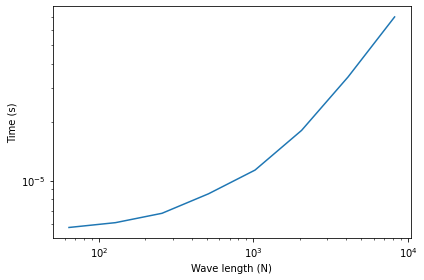
\includegraphics[scale=1]{fig/lab06/lab06_03.png}
		\caption{Время работы метода ДКП scipy.fftpack.dct}
	\end{center}
\end{figure}

Данная реализация довольно быстрая, также она пропорциональна n*log(n)

Построим для наглядности все 3 графика на одном

\begin{lstlisting}[language=Python]
plt.plot(ns, bests, label='analyze1')
plt.plot(ns, bests2, label='analyze2')
plt.plot(ns, bests3, label='fftpack.dct')
loglog = dict(xscale='log', yscale='log')
decorate(xlabel='Wave length (N)', ylabel='Time (s)', **loglog)
\end{lstlisting}

\begin{figure}[H]
	\begin{center}
		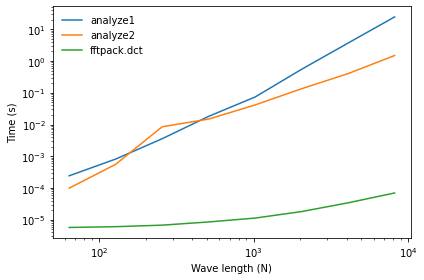
\includegraphics[scale=1]{fig/lab06/lab06_04.png}
		\caption{Время работы различных методов ДКП}
	\end{center}
\end{figure}


\subsection{Упражнение 2}

Реализуем аглоритм ДКП, который предназначен для сжатия звука и изображений. Возьмем звук гитары и выделим из него короткий сегмент

\begin{lstlisting}[language=Python]
if not os.path.exists('469283__matt141141__cm7-dm7-115bpm-loop.wav'):
    !wget https://github.com/sergeyfedorov02/Telecom/raw/main/469283__matt141141__cm7-dm7-115bpm-loop.wav

wave = read_wave('469283__matt141141__cm7-dm7-115bpm-loop.wav')

wave.make_audio()

segment = wave.segment(start = 2, duration = 0.8)
segment.normalize()
segment.make_audio()
\end{lstlisting}

Построим DCT график для данного сегмента

\begin{lstlisting}[language=Python]
segment_dct = segment.make_dct()
segment_dct.plot(high = 4000)
decorate(xlabel='Frequency (Hz)', ylabel='DCT')
\end{lstlisting}

\begin{figure}[H]
	\begin{center}
		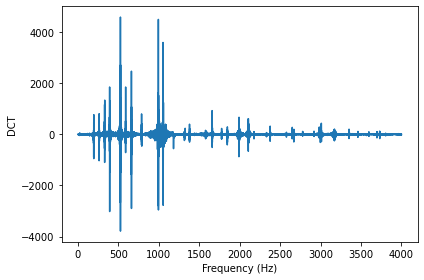
\includegraphics[scale=1]{fig/lab06/lab06_05.png}
		\caption{Спектр сигнала полученный при помощи DCT}
	\end{center}
\end{figure}

Исходя из графика видно, что есть частоты с большой амплитудой. Далее воспользуемся функцией compress, которая берет DCT и режет элементы, которые ниже аргумента thresh и применим её.

\begin{lstlisting}[language=Python]
def compress (dct, thresh = 1):
    count = 0
    for i, amp in enumerate(dct.amps):
        if abs(amp) < thresh:
          dct.hs[i] = 0
          count += 1

    n = len(dct.amps)
    print(count, n, 100 * count / n, sep = '\t')
\end{lstlisting}

\begin{lstlisting}[language=Python]
segment_dct = segment.make_dct()
compress(segment_dct, thresh = 200)
segment_dct.plot(high = 4000)
\end{lstlisting}

65803	66150	99.47543461829176
\begin{figure}[H]
	\begin{center}
		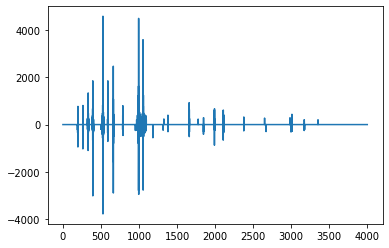
\includegraphics[scale=1]{fig/lab06/lab06_06.png}
		\caption{ДКП после фильтрации}
	\end{center}
\end{figure}

Звучание обратного сигнала

\begin{lstlisting}[language=Python]
segment2 = segment_dct.make_wave()
segment2.make_audio()
\end{lstlisting}


\subsection{Управжнение 3}

Воспользуемся блокнотом phase.ipynb, возьмем оттуда некоторый сегмент звука и повторим эксперименты.

\begin{lstlisting}[language=Python]
from thinkdsp import SquareSignal

signal = SquareSignal(freq=500, offset=0)
wave = signal.make_wave(duration=0.5, framerate=40000)
wave.make_audio()

wave.segment(start=0.005,duration=0.01).plot()
decorate(xlabel='Time (s)')
\end{lstlisting}

\begin{figure}[H]
	\begin{center}
		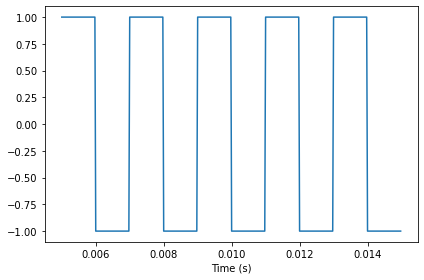
\includegraphics[scale=1]{fig/lab06/lab06_07.png}
		\caption{Выбранный сегмент}
	\end{center}
\end{figure}

\begin{lstlisting}[language=Python]
spect = wave.make_spectrum()
spect.plot()
decorate(xlabel='Frequency (Hz)', ylabel='Amplitude')
\end{lstlisting}

\begin{figure}[H]
	\begin{center}
		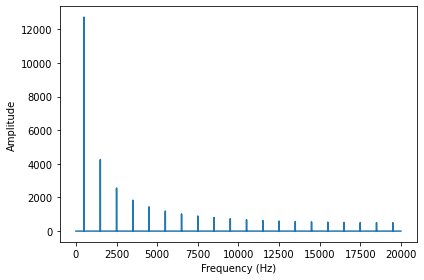
\includegraphics[scale=1]{fig/lab06/lab06_08.png}
		\caption{Спектр сегемента}
	\end{center}
\end{figure}

\begin{lstlisting}[language=Python]
def plot_angle(spectrum, thresh=1):
    angles = spectrum.angles
    angles[spectrum.amps < thresh] = np.nan
    plt.plot(spectrum.fs, angles, 'x')
    decorate(xlabel='Frequency (Hz)', ylabel='Phase (radian)')
    
plot_angle(spect, thresh=0)
\end{lstlisting}

\begin{figure}[H]
	\begin{center}
		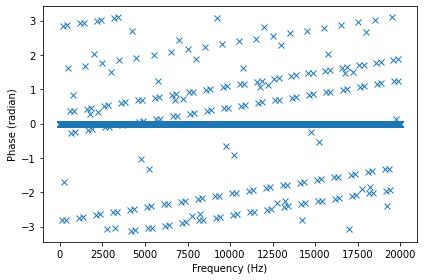
\includegraphics[scale=0.66]{fig/lab06/lab06_09.png}
		\caption{Получившиеся графики}
	\end{center}
\end{figure}

\begin{lstlisting}[language=Python]
plot_angle(spect, thresh=1)
\end{lstlisting}

\begin{figure}[H]
	\begin{center}
		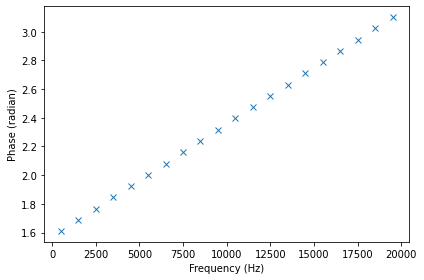
\includegraphics[scale=0.66]{fig/lab06/lab06_10.png}
		\caption{Получившиеся графики}
	\end{center}
\end{figure}


\begin{lstlisting}[language=Python]
def plot_three(spectrum, thresh=1):
    plt.figure(figsize=(10, 4))
    plt.subplot(1,3,1)
    spectrum.plot()
    plt.subplot(1,3,2)
    plot_angle(spectrum, thresh=thresh)
    plt.subplot(1,3,3)
    wave = spectrum.make_wave()
    wave.unbias()
    wave.normalize()
    wave.segment(duration=0.01).plot()
    display(wave.make_audio())
    
plot_three(spect)
\end{lstlisting}

\begin{figure}[H]
	\begin{center}
		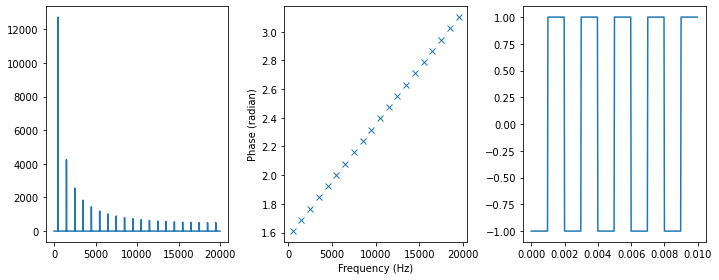
\includegraphics[scale=0.66]{fig/lab06/lab06_11.png}
		\caption{Получившиеся графики}
	\end{center}
\end{figure}

\begin{lstlisting}[language=Python]
def zero_angle(spectrum):
    res = spectrum.copy()
    res.hs = res.amps
    return res
    
spect2 = zero_angle(spect)
plot_three(spect2)
\end{lstlisting}

\begin{figure}[H]
	\begin{center}
		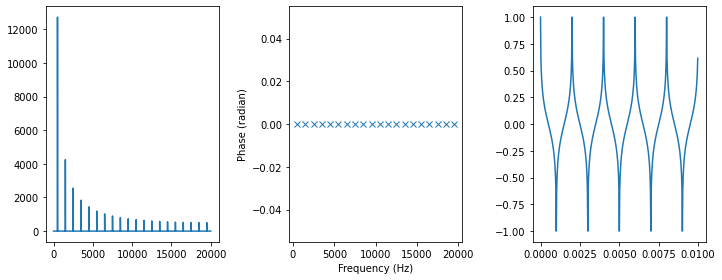
\includegraphics[scale=0.66]{fig/lab06/lab06_12.png}
		\caption{Получившиеся графики}
	\end{center}
\end{figure}

\begin{lstlisting}[language=Python]
def rotate_angle(spectrum, offset):
    res = spectrum.copy()
    res.hs *= np.exp(1j * offset)
    return res
    
spect3 = rotate_angle(spect, 1)
plot_three(spect3)
\end{lstlisting}

\begin{figure}[H]
	\begin{center}
		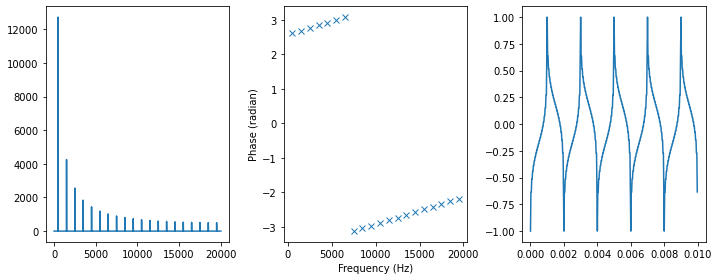
\includegraphics[scale=0.66]{fig/lab06/lab06_13.png}
		\caption{Получившиеся графики}
	\end{center}
\end{figure}

Исходя из графиков видно, что сигнал довольно сильно изменился, но звучание осталось прежним

\begin{lstlisting}[language=Python]
def random_angle(spectrum):
    res = spectrum.copy()
    angles = np.random.uniform(0, PI2, len(spectrum))
    res.hs *= np.exp(1j * angles)
    return res
    
spect4 = random_angle(spect)
plot_three(spect4)
\end{lstlisting}

\begin{figure}[H]
	\begin{center}
		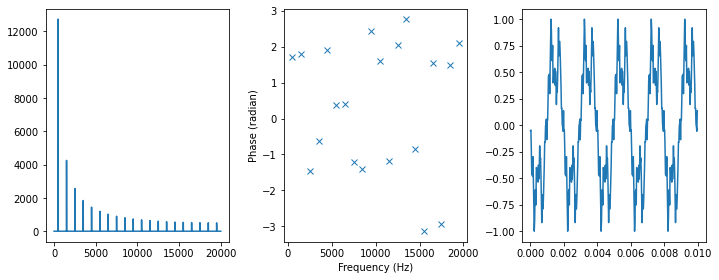
\includegraphics[scale=0.66]{fig/lab06/lab06_14.png}
		\caption{Получившиеся графики}
	\end{center}
\end{figure}

Теперь загрузим собственный звук и проведем тестирование

\begin{lstlisting}[language=Python]
if not os.path.exists('186942__lemoncreme__piano-melody.wav'):
    !wget https://github.com/hotnotHD/Telecom/raw/main/186942__lemoncreme__piano-melody.wav
wave = read_wave('186942__lemoncreme__piano-melody.wav')

wave.make_audio()

segment = wave.segment(start=1.1, duration=0.5)

spect = segment.make_spectrum()
plot_three(spect, thresh=50)
\end{lstlisting}

\begin{figure}[H]
	\begin{center}
		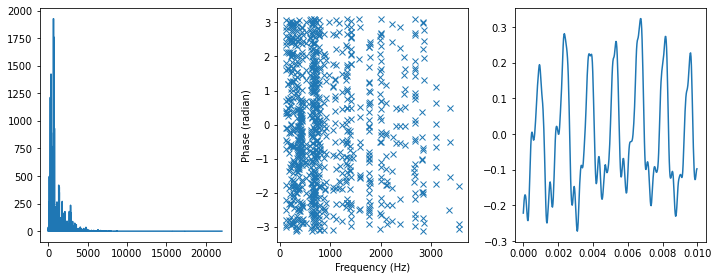
\includegraphics[scale=0.66]{fig/lab06/lab06_15.png}
		\caption{Получившиеся графики}
	\end{center}
\end{figure}

\begin{lstlisting}[language=Python]
spect2 = zero_angle(spect)
plot_three(spect2, thresh=50)
\end{lstlisting}

\begin{figure}[H]
	\begin{center}
		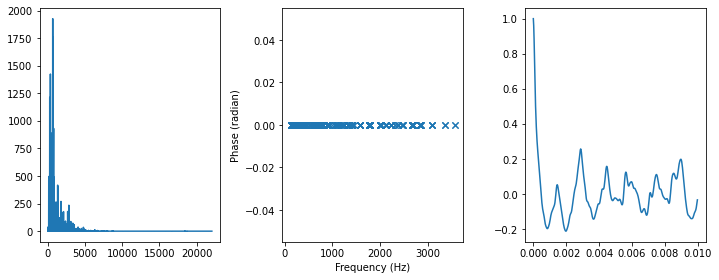
\includegraphics[scale=0.66]{fig/lab06/lab06_16.png}
		\caption{Получившиеся графики}
	\end{center}
\end{figure}

Звучит как в реверсе

\begin{lstlisting}[language=Python]
spect3 = rotate_angle(spect, 1)
plot_three(spect3, thresh=50)
\end{lstlisting}

\begin{figure}[H]
	\begin{center}
		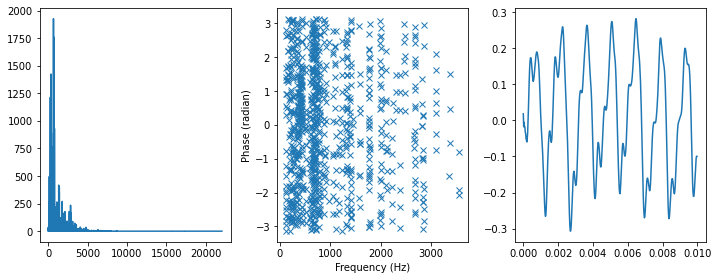
\includegraphics[scale=0.66]{fig/lab06/lab06_17.png}
		\caption{Получившиеся графики}
	\end{center}
\end{figure}

\begin{lstlisting}[language=Python]
spect4 = random_angle(spect)
plot_three(spect4, thresh=50)
\end{lstlisting}

\begin{figure}[H]
	\begin{center}
		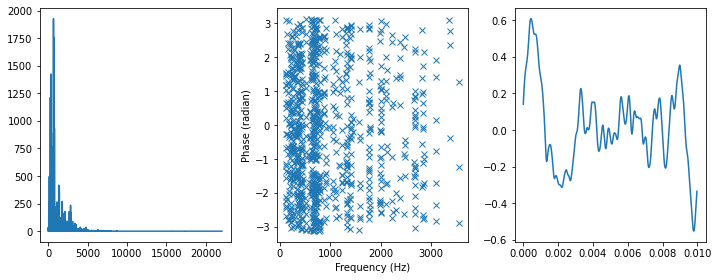
\includegraphics[scale=0.66]{fig/lab06/lab06_18.png}
		\caption{Получившиеся графики}
	\end{center}
\end{figure}

Для звуков с простой гармонической структурой мы не слышим измнения в фазовой структуре, при условии что гармоническая структура неизменна.


\subsection{Вывод}

ДКП применяется в MP3 и соответвующих форматах сжатия музыки, в JPEG, MPEG и так далее. ДКП похоже на ДПФ, использованное в спектральном анализе. Также при помощи ДКП были исследованы свойства звуков с разной структурой.